%%
% Please see https://bitbucket.org/rivanvx/beamer/wiki/Home for obtaining beamer.
%%
\documentclass[hyperref={pdfpagelabels=false}]{beamer}
\usepackage{lmodern}
%\usetheme{CambridgeUS}
\usepackage{color}
\usepackage{listings}

\usepackage{xcolor-solarized}
\usepackage{gitdags}
\usepackage{minted}
\usetheme{netvor}

% Settings
\lstset{basicstyle=\ttfamily,
  showstringspaces=false,
  frame=single
}

% definition of diff language
\lstdefinelanguage{diff}{
  morecomment=[f][\color{blue}]{@@},     % group identifier
  morecomment=[f][\color{red}]-,         % deleted lines 
  morecomment=[f][\color{green}]+,       % added lines
  morecomment=[f][\color{magenta}]{---}, % Diff header lines (must appear after +,-)
  morecomment=[f][\color{magenta}]{+++},
}


\title{git basics}  
\author{Michal \v Stembera} 
\titlegraphic{
\includegraphics[height=0.10\textheight]{logo_netvor}}
\date{\today} 

% TITLEPAGE
\begin{document}
\begin{frame}
	\titlepage
\end{frame} 

\begin{frame}
\frametitle{Table of contents}
\tableofcontents
\end{frame} 

% GIT INIT
\begin{frame}[fragile]
\frametitle{Getting git repository}
	\begin{lstlisting}[language=bash, caption={Creating new repository}]
	git init git-presentation-repo
	\end{lstlisting}

	\begin{lstlisting}[language=bash, caption={Clone remote repository}]
	git clone\
	  https://github.com/stemberamichal/Perfect
	\end{lstlisting}
\end{frame} 

% GIT INIT - CONSEQUENCES
\begin{frame}[fragile]
\frametitle{Initialized repository}
	\begin{columns}
		\begin{column}{0.6\textwidth}
			What we did:
			\begin{itemize}
				\item Folder git-presentation-repo
				\item Subfolder .git with basic content
				\item Branch master
			\end{itemize}	
			What we did not do:
			\begin{itemize}
				\item Not created tracked files or commits
				\item Not added remote repository
			\end{itemize}
			Verify:
			\begin{lstlisting}[language=bash, caption={List all folders and files}]
				find .
			\end{lstlisting}
		\end{column}
		\begin{column}{0.4\textwidth}
			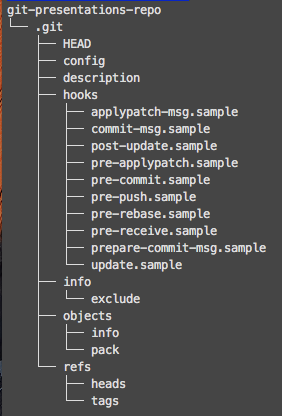
\includegraphics[width=\textwidth]{empty-repo-tree}
		\end{column}	
	\end{columns}
\end{frame} 

% WHAT IS GIT
\section{What is git} 
\subsection{Subsection no.1.1}
\begin{frame}
\frametitle{Version Control System (VCS)}
\begin{columns}
\begin{column}{0.4\textwidth}
	\begin{itemize}
		\item Distributed version control
		\item Each client has its copy of history
		\item Database can be altered offline
	\end{itemize}
\end{column}
\begin{column}{0.6\textwidth}  %%<--- here
    \begin{center}
     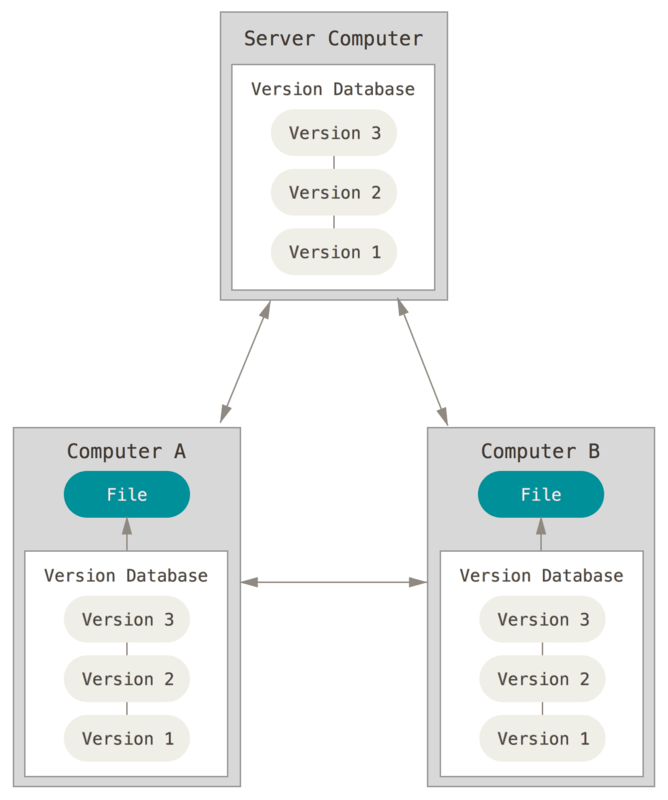
\includegraphics[width=0.6\textwidth]{distributed}
     \end{center}
\end{column} 
\end{columns}
\end{frame}

% ADDING REMOTE
\begin{frame}[fragile]
\frametitle{Adding remote}
	\begin{lstlisting}[language=bash, caption={Add remote called origin}]
	git remote add origin\
	  https://github.com/stemberamichal/Perfect
	\end{lstlisting}
	
	\begin{lstlisting}[language=bash, caption={Add another remote}]
	git remote add perfect\
	  https://github.com/PerfectlySoft/Perfect
	\end{lstlisting}
\end{frame}

% SYNCHRONIZING CHANGES
\begin{frame}[fragile]
\frametitle{Fetch repositories}
\begin{figure}
    \begin{tikzpicture}
      \gitDAG[grow right sep = 2em]{
        A -- B -- { 
          C,
          D -- E,
        }
      };
      % Local branch
      \gitbranch
      	[master]
      	{master}
      	{above=of A}
      	{A}
      % Remote branch
		\pause\gitremotebranch
        [origmaster]    % node name
        {origin/master} % node text
        {above=of C}    % node placement
        {C}             % target
      \pause\gitremotebranch
        [perfmaster]    % node name
        {perfect/master} % node text
        {above=of E}    % node placement
        {E}             % target
    \end{tikzpicture}
\end{figure}
	% git fetch origin
	\begin{lstlisting}[language=bash]
	git fetch origin
	\end{lstlisting}
	% git fetch perfect 2+
	\begin{onlyenv}<2->
	\begin{lstlisting}[language=bash]
	git fetch perfect
	\end{lstlisting}
	\end{onlyenv}
	% git fetch -all 3+
	\begin{onlyenv}<3->
	\begin{lstlisting}[language=bash]
		git fetch --all
	\end{lstlisting}
	\end{onlyenv}
\end{frame}

% INTERNAL REPRESENTATIONS
\begin{frame}
\frametitle{Deltas or snapshot}
\begin{columns}
\begin{column}{0.3\textwidth}
	\begin{itemize}
		\item Exposed as deltas
		\vspace{0.1\textheight}
		\item Internally stored as snapshots
	\end{itemize}
\end{column}
\begin{column}{0.7\textwidth}  %%<--- here
	\begin{center}
    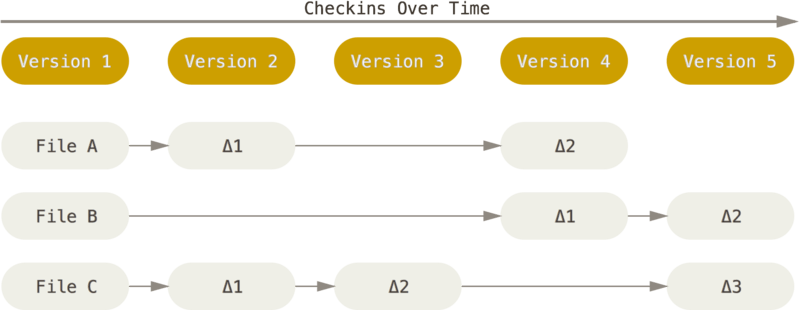
\includegraphics[width=0.8\textwidth]{deltas}
    \vspace{2em}
    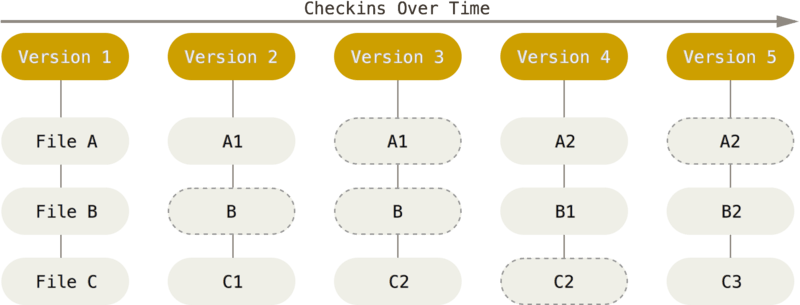
\includegraphics[width=0.8\textwidth]{snapshots}
    \end{center}
\end{column}
\end{columns}
\end{frame}

% GIT STATES
\begin{frame}
\frametitle{The Three States}
	\begin{description}[Three states]
		\item [Working directory] Current changes to the filesystem
		\item [Staging area]Changes marked for commit
		\item [Commited] Internally stored as snapshots
	\end{description}
    \begin{center}
    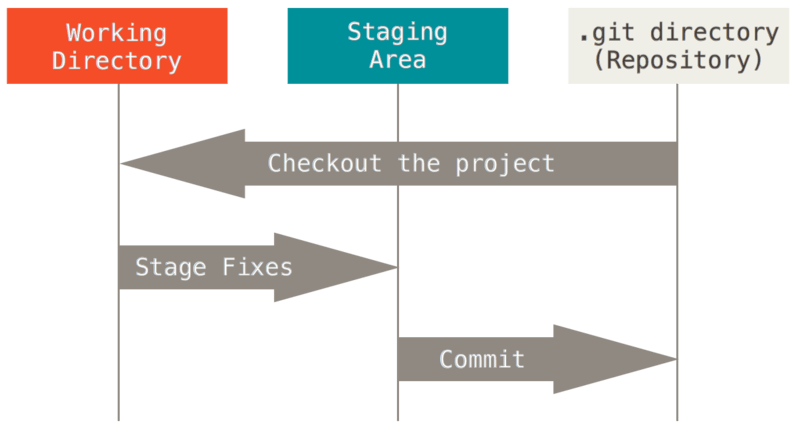
\includegraphics[width=0.6\textwidth]{areas}
    \end{center}
\end{frame}

\begin{frame}[fragile]
	\lstinputlisting[language=diff]{basics.diff}
\end{frame}

\begin{frame}
\section{Section no. 2} 
\subsection{Lists I}
\begin{columns}[T]
\column{.5\textwidth}
 \visible<1->{\begin{figure}
    \centering
    \begin{tikzpicture}
      % Commit DAG
      \gitDAG[grow right sep = 2em]{
        A -- B -- { 
          C,
          D -- E,
        }
      };
      % Tag reference
      \gittag
        [v0p1]       % node name
        {v0.1}       % node text
        {above=of A} % node placement
        {A}          % target
      % Remote branch
      \gitremotebranch
        [origmaster]    % node name
        {origin/master} % node text
        {above=of C}    % node placement
        {C}             % target
      % Branch
      \gitbranch
        {master}     % node name and text 
        {above=of E} % node placement
        {E}          % target
      % HEAD reference
      \gitHEAD
        {above=of master} % node placement
        {master}          % target
    \end{tikzpicture}
\end{figure}}
\visible<2->{\begin{figure}
    \centering
    \begin{tikzpicture}
      % Commit DAG
      \gitDAG[grow right sep = 2em]{
        A -- B -- { 
          C,
          D -- E,
        }
      };
      % Tag reference
      \gittag
        [v0p1]       % node name
        {v0.1}       % node text
        {above=of A} % node placement
        {A}          % target
      % Remote branch
      \gitremotebranch
        [origmaster]    % node name
        {origin/master} % node text
        {above=of C}    % node placement
        {C}             % target
      % Branch
      \gitbranch
        {master}     % node name and text 
        {above=of E} % node placement
        {E}          % target
      % HEAD reference
      \gitHEAD
        {above=of master} % node placement
        {master}          % target
    \end{tikzpicture}
\end{figure}}
\column{.5\textwidth}
\visible<3->{\begin{figure}
    \centering
    \begin{tikzpicture}
      % Commit DAG
      \gitDAG[grow right sep = 2em]{
        A -- B -- { 
          C,
          D -- E,
        }
      };
      % Tag reference
      \gittag
        [v0p1]       % node name
        {v0.1}       % node text
        {above=of A} % node placement
        {A}          % target
      % Remote branch
      \gitremotebranch
        [origmaster]    % node name
        {origin/master} % node text
        {above=of C}    % node placement
        {C}             % target
      % Branch
      \gitbranch
        {master}     % node name and text 
        {above=of E} % node placement
        {E}          % target
      % HEAD reference
      \gitHEAD
        {above=of master} % node placement
        {master}          % target
    \end{tikzpicture}
\end{figure}}
\end{columns}
\end{frame}

\end{document}
